% !TeX root = RJwrapper.tex
\title{detourr: An R Package extending \{tourr\} with \{HTMLWidgets\}}
\author{by Casper Hart and Earo Wang}

\maketitle

\abstract{%
An abstract of less than 150 words.
}

\hypertarget{introduction}{%
\section{Introduction}\label{introduction}}

Multivariate data often contains interesting features that we would like
to uncover when performing exploratory data analysis. These features
include clusters of points, outliers, linear dependiencies, non-linear
relationships, and low-dimensional substructures, and can often remain
hidden when using static visualizations such as histograms and
scatterplot matrices \citep{tours}.

A common method for exploring multivariate data is the tour, where we
take a sequence of \(d < p\)-dimensional projections of our data and
interpolate between them to create an animation. These animations allow
us to view the data from many different angles, and helps us to uncover
the features mentioned above.

The \CRANpkg{tourr} package in R produces tours of multivariate data.
The animations produced by \CRANpkg{tourr} can be viewed using the R
graphics device, passed to \href{https://github.com/ggobi}{\pkg{GGobi}},
or saved to disk \citep{tourr2011}.

This paper introduces the \pkg{detourr} package, which extends
\CRANpkg{tourr} with interactive web-based visualisations using
\CRANpkg{HTMLWidgets}. We begin with a brief review of the
\CRANpkg{tourr} package, and how we've built upon it. We will then
include a series of examples to showcase the functionality of
\pkg{detourr}, including interactive features like brushing, selection,
tooltips, and timeline controls. We will also cover integration with the
\CRANpkg{crosstalk} for linking different visuals, performance
considerations, and lastly the project structure and how to contribute.

\hypertarget{background-tourr}{%
\section{Background: \{tourr\}}\label{background-tourr}}

The \CRANpkg{tourr} package in R is designed to be extensible and is
intended to provide a testbed for tour research \citep{tourr2011}. One
way this extensibility is achieved is by separating out the tour
generators (e.g.~\texttt{grand\_tour}, \texttt{little\_tour}) from the
display methods (e.g.~\texttt{display\_xy}, \texttt{display\_depth}).

For example, the following code produces a 2-d tour which is displayed
as a scatter plot using the R Graphics device:

\begin{Schunk}
\begin{Sinput}
animate(flea[, 1:6],
  grand_tour(d = 2),
  display = display_xy()
)
\end{Sinput}
\end{Schunk}

A similar animation can be rendered as a GIF like in the following code:

\begin{Schunk}
\begin{Sinput}
render_gif(
  flea[, 1:6],
  grand_tour(d = 2),
  display_xy(),
  "img/flea.gif"
)
\end{Sinput}
\end{Schunk}

\begin{Schunk}
\begin{Soutput}
#> target_dist - cur_dist: 0 
#> generation:  dist =   1.540576
\end{Soutput}
\begin{Soutput}
#> target_dist - cur_dist: 1.540576
\end{Soutput}
\begin{figure}
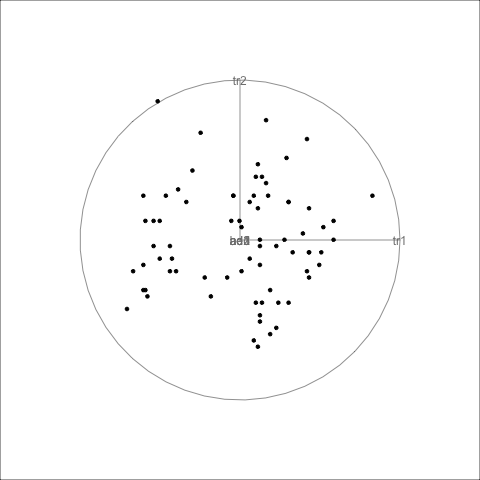
\includegraphics[width=\textwidth]{img/flea} \caption[A grand tourr of the flea data rendered as an x-y scatterplot]{A grand tourr of the flea data rendered as an x-y scatterplot.}\label{fig:flea-tourr}
\end{figure}
\end{Schunk}

In general, the call used in \CRANpkg{tourr} has the form
\citep{tourr2011}:

\begin{Schunk}
\begin{Sinput}
tour_function(data, tour_path, display_method)
\end{Sinput}
\end{Schunk}

\hypertarget{detourr}{%
\section{\{detourr\}}\label{detourr}}

The \pkg{detourr} package extends \CRANpkg{tourr} and has a similar
structure, but with a few important differences:

\begin{itemize}
\tightlist
\item
  Only one tour function is currently supported: \texttt{animate\_tour}
\item
  \pkg{detourr} has it's own display methods (\texttt{display\_scatter})
  which are not compatible with \CRANpkg{tourr}.
\item
  Input data must be provided as a data frame, not a matrix.
\end{itemize}

\begin{Schunk}
\begin{Sinput}
animate_tour(flea,
  tour_path = grand_tour(2),
  display = display_scatter(colour = species)
)
\end{Sinput}
\end{Schunk}

\hypertarget{interactivity}{%
\section{Interactivity}\label{interactivity}}

Brushing, selection, hovering / labels

\hypertarget{crosstalk-integration}{%
\section{Crosstalk Integration}\label{crosstalk-integration}}

Javascript JIT / matrix multiplication

drawing: HTML Canvas vs SVG

sleep

\hypertarget{performance-considerations}{%
\section{Performance Considerations}\label{performance-considerations}}

Javascript JIT / matrix multiplication

drawing: HTML Canvas vs SVG

sleep

\hypertarget{summary}{%
\section{Summary}\label{summary}}

We have displayed various tooltips that are available in the package
\pkg{ToOoOlTiPs}.

\bibliography{detourr.bib}

\address{%
Casper Hart\\
University of Auckland\\%
Department of Statistics\\
%
%
%
\href{mailto:casperhart93@gmail.com}{\nolinkurl{casperhart93@gmail.com}}%
}

\address{%
Earo Wang\\
University of Auckland\\%
Department of Statistics\\
%
%
%
\href{mailto:earo.wang@auckland.ac.nz}{\nolinkurl{earo.wang@auckland.ac.nz}}%
}
